\documentclass{article}

\usepackage{graphicx}
\usepackage{tikz}
\usepackage{tikzsymbols}
\usetikzlibrary{calc,patterns,shapes.geometric}
\pagestyle{empty}
\usepackage[margin=0pt]{geometry}
\geometry{papersize={14in,12in}}

\def\centerarc[#1](#2)(#3:#4:#5){\draw[#1] ($(#2)+({#5*cos(#3)},{#5*sin(#3)})$) arc (#3:#4:#5);}

\begin{document}
	\begin{figure}
		\centering
		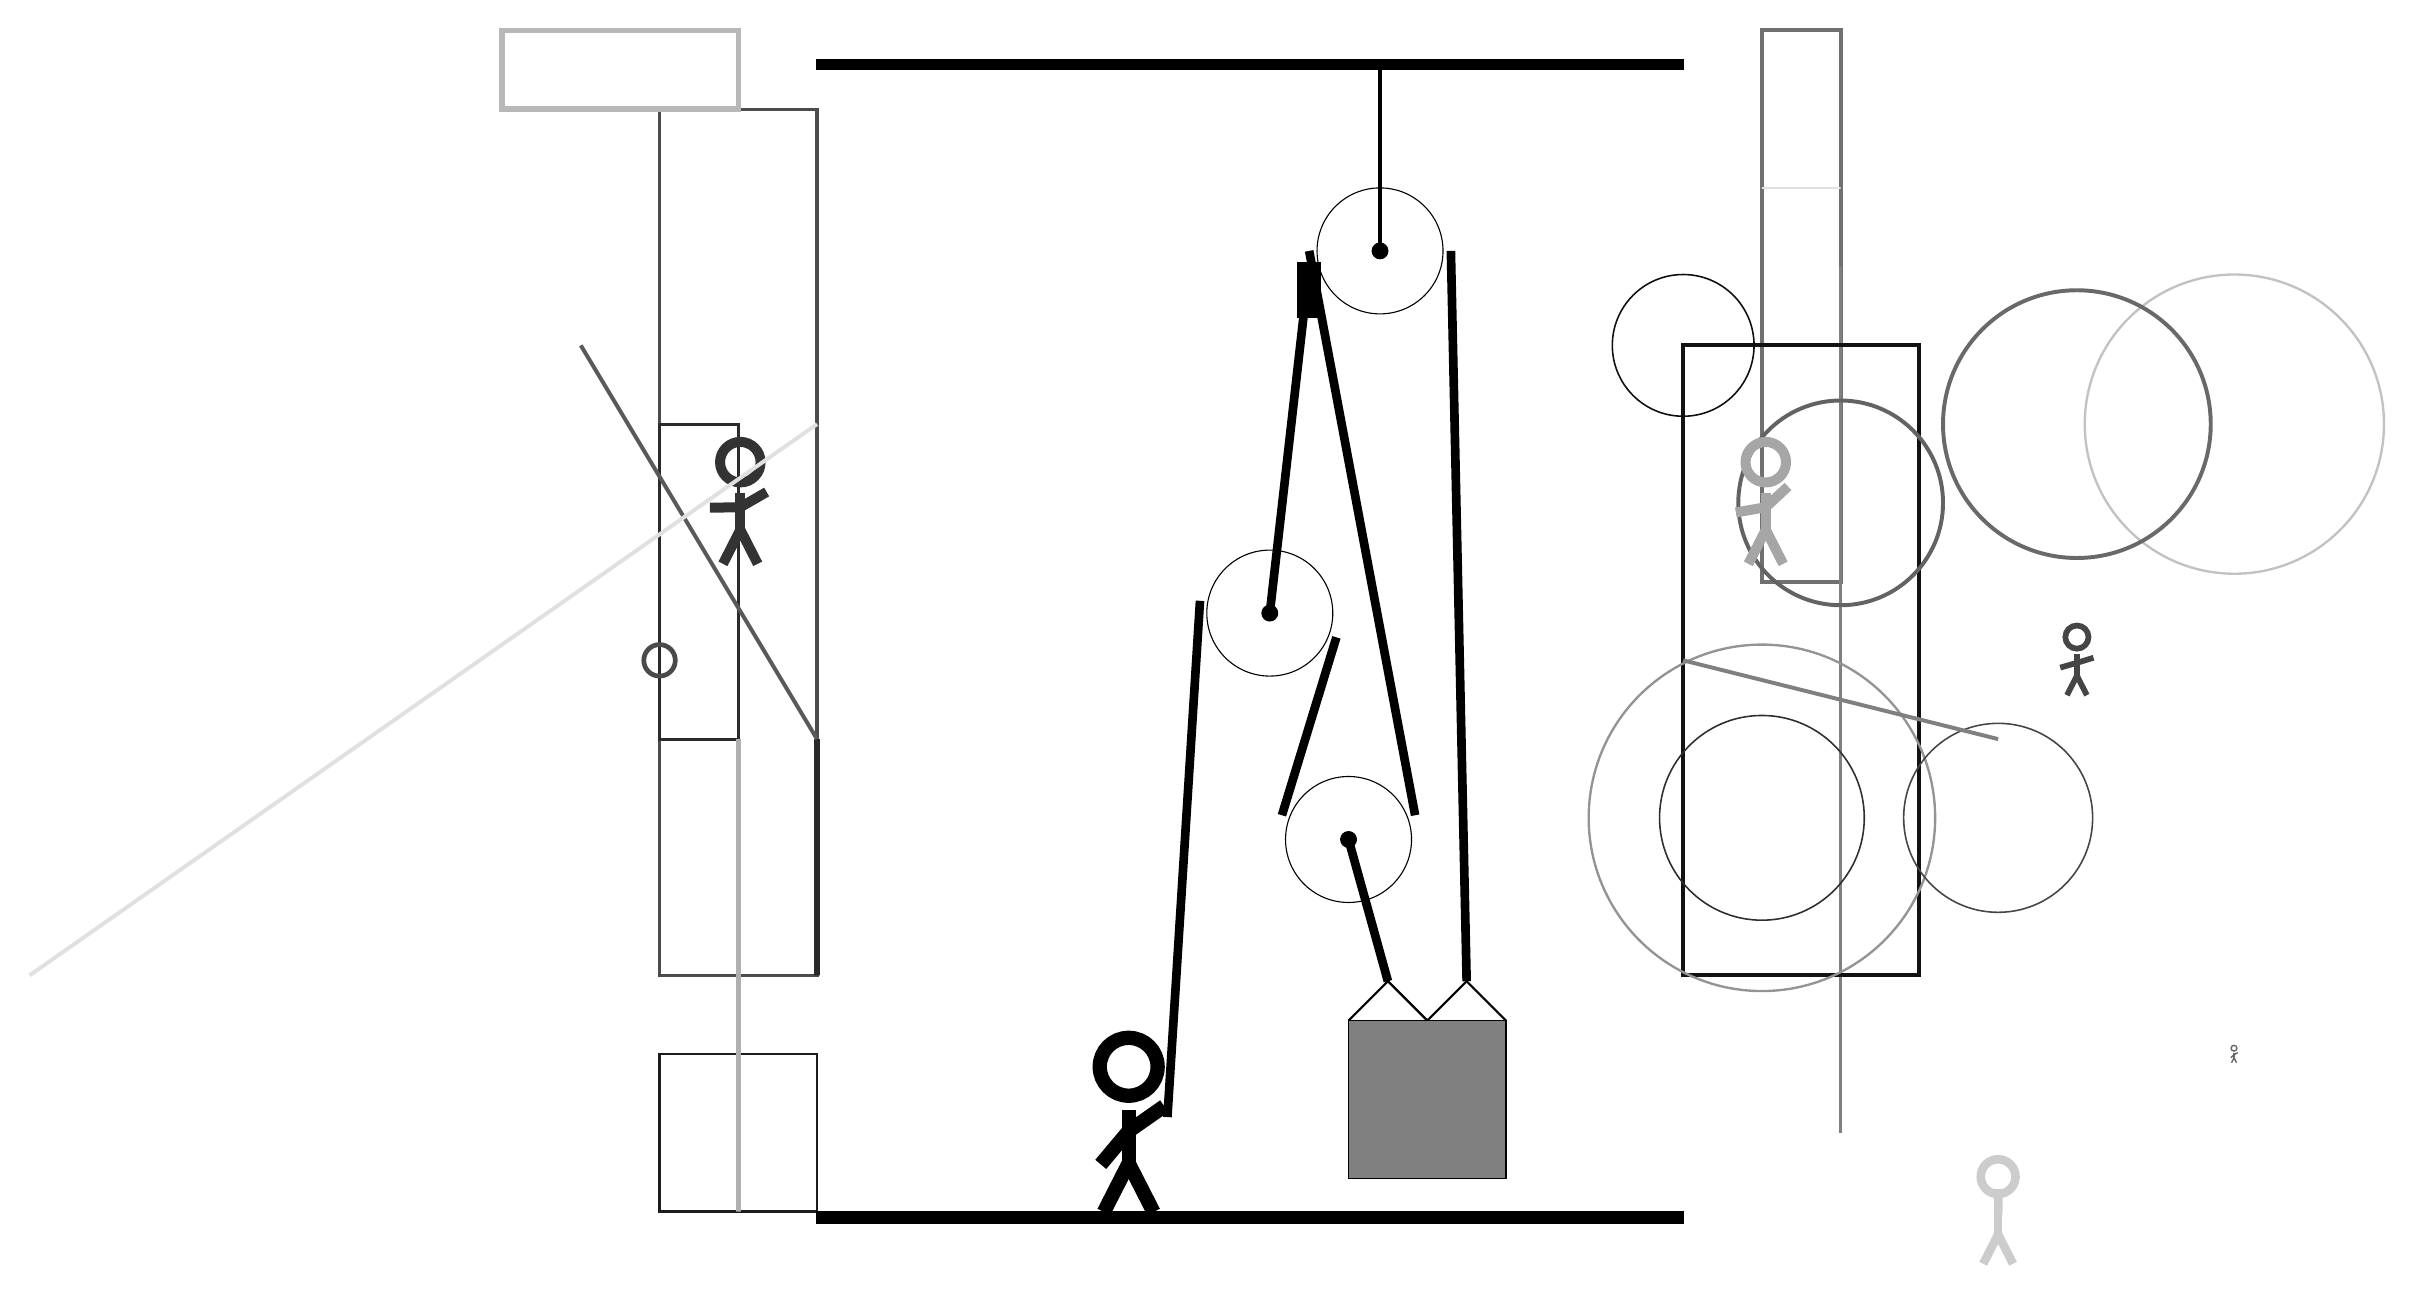
\begin{tikzpicture}
			%%%%% START %%%%%
			
			\draw[fill=black] (-6, 11.5) rectangle (5, 11.625);
			
			\draw[line width=0.5mm, color=black!56] (6, 12) rectangle (7, 5);
			
			\draw[line width=0.4mm, color=black!70] (-6, 0) rectangle (-8, 11);
			\draw[line width=0.3mm, color=black!50] (7, -2) rectangle (7, 9);
			\draw[line width=0.5mm, color=black!93] (5, 0) rectangle (8, 8);
			\draw[line width=0.4mm, color=black!83] (-7, 3) rectangle (-8, 7);
			
			\draw [line width=0.6mm, color=black!71](-8, 4) circle (0.2);
			\draw [line width=0.2mm, color=black!82](6, 2) circle (1.3);
			
			\draw[line width=0.7mm, color=black!84] (-6, 3) rectangle (-6, 0);
			\draw [line width=0.2mm, color=black!94](5, 8) circle (0.9);
			\node[line width=0.2mm, color=black!80] at (-7, 6) {\Strichmaxerl[7][1][30]};
			\draw [line width=0.3mm, color=black!42](6, 2) circle (2.2);
			
			\draw[line width=0.5mm, color=black!65](-9, 8) -- (-6, 3);
			\node[line width=0.7mm, color=black!73] at (10, 4) {\Strichmaxerl[4][16][17]};
			
			\draw [line width=0.5mm, color=black!61](7, 6) circle (1.3);
			\node[line width=0.4mm, color=black!35] at (6, 6) {\Strichmaxerl[7][10][43]};
			\draw[line width=0.5mm, color=black!12](-6, 7) -- (-16, 0);
			
			\draw [line width=0.3mm, color=black!24](12, 7) circle (1.9);
			\draw[line width=0.2mm, color=black!12] (7, 10) rectangle (6, 10);
			\draw [line width=0.5mm, color=black!59](10, 7) circle (1.7);
			
			\draw [line width=0.2mm, color=black!73](9, 2) circle (1.2);
			\draw[line width=0.5mm, color=black!50](5, 4) -- (9, 3);
			
			\draw[line width=0.3mm, color=black!89] (-6, -1) rectangle (-8, -3);
			\node[line width=0.5mm, color=black!20] at (9, -3) {\Strichmaxerl[6][90][89]};
			\draw[line width=0.7mm, color=black!28] (-7, 12) rectangle (-10, 11);
			\draw[line width=0.6mm, color=black!31] (-7, -3) rectangle (-7, 3);
			\node[line width=0.6mm, color=black!59] at (12, -1) {\Strichmaxerl[1][43][27]};
			
			
			\draw (-0.25, 4.6) circle (0.8);
			\draw[fill=black] (-0.25, 4.6) circle (0.1);
			
			\draw (0.75, 1.725) circle (0.8);
			\draw[fill=black] (0.75, 1.725) circle (0.1);
			
			\draw (1.15, 9.2) circle (0.8);
			\draw[fill=black] (1.15, 9.2) circle (0.1);
			\draw[very thick] (1.15, 9.2) -- (1.15, 11.5);
			
			\draw[thick]  (0.75, -0.575) -- (1.25, -0.075) -- (1.75, -0.575) -- (2.25, -0.075) -- (2.75, -0.575);
			\draw[fill=black!50] (0.75, -0.575) rectangle (2.75, -2.575);
			
			\draw[line width=1.1mm] (-0.25, 4.6) -- (0.25, 9.0);
			\draw[line width=1.1mm, fill=black](0.15, 8.4) rectangle (0.35, 9.0);
			\draw[line width=1.1mm] (-1.55, -1.8) -- (-1.1363, 4.7562);
			\centerarc[line width=1.1mm](-0.25, 4.6)(-20:170:0.9);
			\draw[line width=1.1mm] (0.5957, 4.2922) -- (-0.0957, 2.0328);
			\centerarc[line width=1.1mm](0.75, 1.725)(160:380:0.9);
			\draw[line width=1.1mm] (1.5957, 2.0328) -- (0.25, 9.2);
			\draw[line width=1.1mm](0.75, 1.725) -- (1.25, -0.075);
			\centerarc[line width=1.1mm](1.15, 9.2)(0:180:0.9);
			\draw[line width=1.1mm] (2.05, 9.2) -- (2.25, -0.075);
			
			\node at (-2, -1.9) {\Strichmaxerl[10][50][35]};
			
			\draw[fill=black] (-6, -3) rectangle (5, -3.15);
			
			%%%%% END %%%%%
		\end{tikzpicture}
	\end{figure}	
\end{document}